\begin{frame}{decompiler}
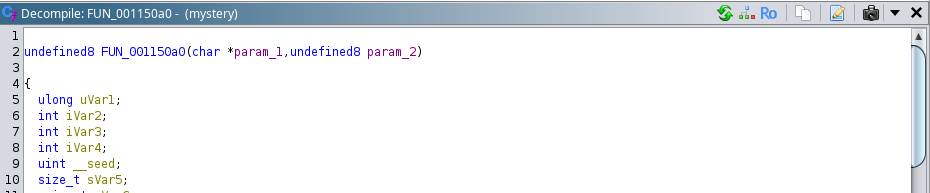
\includegraphics[width=0.9\textwidth]{../re-tools/decomp-top} \\
\ldots  \\
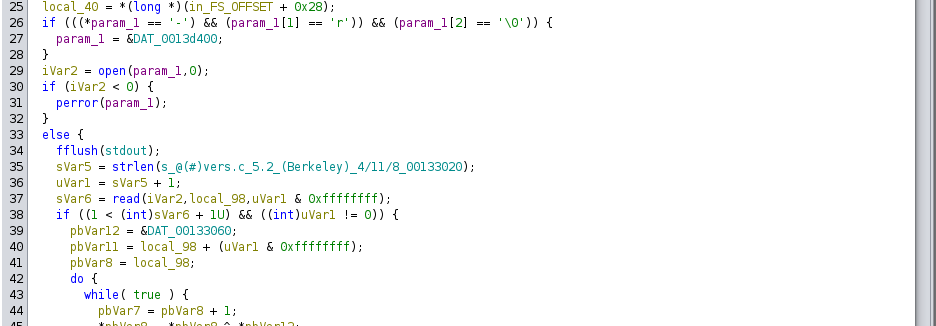
\includegraphics[width=0.9\textwidth]{../re-tools/decomp-rest}
\end{frame}

\begin{frame}{refining decompile (1)}
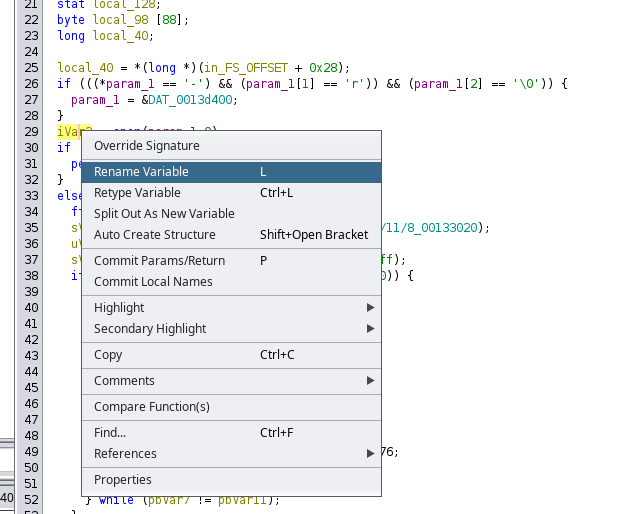
\includegraphics[width=0.9\textwidth]{../re-tools/ghidra-edit-var-decomp}
\end{frame}

\begin{frame}{refining decompile (2)}
    \begin{itemize}
    \item can setup names, types for functions
    \item types can include marking array
        \begin{itemize}
        \item Ghidra doesn't seem great at inferring this all the time
        \end{itemize}
    \vspace{.5cm}
    \item also for local/global variables
        \begin{itemize}
        \item for globals, can right-click in listing view too
        \end{itemize}
    \end{itemize}
\end{frame}

